\label{sec:results}
\providecommand{\nym}{\textbf{[NOT YET MEASURED]}}
\providecommand{\xh}{x_{\mathrm{h}}}
\tikzset{
  resbox/.style={draw,rounded corners=2pt,fill=gray!12,align=center,font=\footnotesize,minimum height=7mm,inner sep=3pt},
  resdark/.style={draw,rounded corners=2pt,fill=gray!30,align=center,font=\footnotesize,minimum height=7mm,inner sep=3pt},
  resarr/.style={-{Stealth[length=2.2mm]},thick}
}

\subsection{Summary of results achieved} % REQUIRED HEADING
\label{sec:res-summary}

This section documents how the system is to be qualified against the requirements R1 to R6 and the field conditions FC1 and FC2 of the approved project proposal, and reports the results that exist.
No new measurements were taken for this report.
The figures below are design-stage or previous-run figures obtained on a development laptop, not on the ODROID N2+, and each carries the caveat that limits its value.
Every quantity that has not been measured is marked \nym{} and accompanied by its protocol and the outcome that the design predicts.
Four status labels are used in Table~\ref{tab:res-summary}: \emph{Met}, \emph{Partially met} (evidence exists but is circular, optimistic or incomplete), \emph{Not met} and \emph{Not yet measured}.

\begin{table}[h]
\centering
\fontsize{10}{12}\selectfont
\begin{tabularx}{\linewidth}{|>{\raggedright\arraybackslash}p{4.6cm}|>{\raggedright\arraybackslash}X|>{\raggedright\arraybackslash}p{2.3cm}|}
\hline
\textbf{Intended outcome} & \textbf{Actual outcome} & \textbf{Location in report} \\
\hline
\multicolumn{3}{|l|}{\textbf{Core mission requirements and specifications}} \\
\hline
R1: Reproduce desired text in the style of any writer of the training set with at least 85\% character accuracy and 85\% stylistic correlation; a reproduced sentence must visibly match the input text in at least 85\% of its characters. &
\textbf{Partially met.} Design-stage evaluations with the same judges that drive the best-of-$N$ search gave 81.6\% (direct) and 81.4\% (G-code) character accuracy and 97.5\%/95.8\% writer identification at $N=14$; a scoped run on two writers gave 92.9\% character accuracy. All figures are circular. Independent character accuracy, style correlation and overlay distances: \nym{}. &
Qualification test 1 \\
\hline
R2: Decode the text of handwritten pages and identify the writer with an overall accuracy of at least 95\%. &
\textbf{Not met for text; overall not yet measured.} Recogniser character accuracy 91.82\% (general test set) and 89.64\% (personal validation lines); writer identification 100\% on real validation pages (optimistic, line-level split). Overall accuracy on held-out photographed pages: \nym{}. &
Qualification test 2 \\
\hline
R3: Reproduce text at no more than 4~s per character. &
\textbf{Partially met (not measured on the target hardware).} Synthesis took about 2.8~s per character (105~s for 38 characters, loaded laptop) with best-of-$N$; a three-try synthesis took 5 to 7~s. Physical writing time: \nym{}; the generator model predicts 2.4 to 2.8~s per character. &
Qualification test 3 \\
\hline
R4: Identify the writer and decode the text within $2+0.025x$~s for $x$ characters. &
\textbf{Not met.} Segmentation alone took 35 to 57~s per photograph in pure Python on the laptop (budget 2~s); the recogniser took 65 to 75~ms per character (budget 25~ms). On the ODROID N2+: \nym{}. &
Qualification test 4 \\
\hline
R5: Absolute gantry positional error of at most 0.5~mm. &
\textbf{Not yet measured.} Step resolution 12.5~$\mu$m (derived). The X-axis calibration reached the first end-stop, but the direction pin was not observed to change level on reversal; the fault was unresolved. &
Qualification test 5 \\
\hline
R6: At least 10 writing styles trained and stored permanently. &
\textbf{Met for storage.} Ten writers (eight database, two personal) are stored as JSON style profiles with trained weights, and the server lists ten. Restart persistence and a random-writer demonstration: \nym{}. &
Qualification test 6 \\
\hline
\multicolumn{3}{|l|}{\textbf{Field condition requirements and specifications}} \\
\hline
FC1: Operation in well-lit areas, 400 to 1000~lux. &
\textbf{Not yet measured.} No illuminance measurement was recorded. &
Section~\ref{sec:res-fc} \\
\hline
FC2: Operation on a stable, level, vibration-free surface. &
\textbf{Not yet measured.} No level or vibration check was recorded. &
Section~\ref{sec:res-fc} \\
\hline
\end{tabularx}
\caption{Summary of results achieved.}
\label{tab:res-summary}
\end{table}

Only R6 can be reported as met; R4 shows a clear measured shortfall, and R5 could not be assessed because the hardware bring-up was not completed.
Causes and remedies are analysed in Section~\ref{sec:discussion}.

\subsection{Qualification tests} % REQUIRED HEADING
\label{sec:res-qtp}

This subsection summarises, for each requirement, the test that is to prove it on the integrated system, in the order of importance of the proposal.
The detailed step lists, metric definitions and data sheets are given in the Appendix (Section ``Extended qualification-test protocols'').
Proportions are reported with a 95\% Wilson score interval \cite{wilson1927},
\begin{equation}
\label{eq:res-wilson}
\hat p_{\pm}=\frac{\hat p+\dfrac{z^2}{2n}\pm z\sqrt{\dfrac{\hat p(1-\hat p)}{n}+\dfrac{z^2}{4n^2}}}{1+\dfrac{z^2}{n}},\qquad \hat p=\frac{k}{n},
\end{equation}
where $k$ is the number of successes in $n$ trials and $z=1.96$; it stays valid near 0\% and 100\%.
Characters of one page are not independent, so a page-level percentile bootstrap with 2000 resamples \cite{efron1979} is used for accuracies.
A requirement is declared met only if the lower confidence bound exceeds the target.
Character accuracy uses the Levenshtein distance \cite{levenshtein1966} $d_L(h,r)$ between hypothesis $h$ and reference $r$ (minimum number of insertions, deletions and substitutions),
\begin{equation}
\label{eq:res-cacc}
A_{\mathrm{c}}=1-\frac{d_L(h,r)}{\lvert r\rvert},
\end{equation}
summed over all sentences, where $\lvert r\rvert$ is the reference length.
All random choices use recorded seeds.

%%%%%%%%%%%%%%%%%%%%%%%%%%%%%%%%%%%%%%%%%%%%%%%%%%%%%%%%%%%%%%%%%%%%%%%%%%%%%%%%%

\medskip
    \QualificationTest{Reproduction fidelity of the synthesised handwriting (R1)}
\label{sec:res-qtp1}

        \QualificationSection{Objectives of the test or experiment}

            The test is to prove at least 85\% character accuracy and 85\% stylistic correlation.
            The existing evidence is circular, because the networks that select the best of $N$ candidates also score the result; the test therefore uses judges outside the search.

        \QualificationSection{Equipment used}

            The ODROID N2+ with the server and ten stored profiles, the gantry for the demonstration, a separate evaluation program (not importing the synthesiser or its judges), the base recognition checkpoint that is not used in the search, and printed worksheets for a blind human panel.

        \QualificationSection{Test setup and experimental parameters}

            Ten writers, 5 novel sentences of 30 to 60 characters each, 3 seeds, $N=14$, direct and G-code rendering: 150 renderings per condition.
            Sub-test (a): the base recogniser and a blind panel of 8 raters (30 synthesised and 10 genuine control lines, agreement by Fleiss' kappa \cite{fleiss1971}) give character accuracy.
            Sub-test (b): seven hand-crafted style features from one deterministic extractor are computed on held-out real pages and on renderings, and the Pearson correlation $\rho$ of the pooled $z$-scored vectors and a nearest-centroid writer retrieval are reported.
            Sub-test (c): the sentence a writer actually wrote is synthesised in that writer's style, both images are normalised to a common x-height $\xh$, and the chamfer and modified Hausdorff distances \cite{dubuisson1994} are compared between 40 matched and 360 mismatched pairs by rank-1 retrieval and the area under the receiver operating characteristic curve (AUC; 0.5 means no writer information).
            Sub-test (d): the demonstration of the proposal, with 85\% of the produced characters visibly matching.
            The definitions (Equations~\ref{eq:res-kappa} to~\ref{eq:res-auc}), features (Table~\ref{tab:res-features}), worksheet (Table~\ref{tab:res-panel}) and the procedure of Figure~\ref{fig:res-overlay} are in the Appendix.

        \QualificationSection{Steps followed in the test or experiment}

            The held-out pages are fixed and the system frozen; the renderings are produced on the ODROID N2+; sub-tests (a) to (d) are then evaluated in order (numbered steps in the Appendix); the confusion matrix, overlay figures and intervals are produced from stored outputs.

        \QualificationSection{Results or measurements}

            Only design-stage figures exist (Table~\ref{tab:res-r1}); the text and writer figures are circular.
            They are compared with the targets in Figure~\ref{fig:res-bars}.

\begin{table}[h]
\centering
\fontsize{10}{12}\selectfont
\begin{tabularx}{\linewidth}{|>{\raggedright\arraybackslash}p{4.7cm}|>{\raggedright\arraybackslash}X|}
\hline
\textbf{Measure} & \textbf{Established figure and caveat, or status} \\
\hline
Character accuracy, search judges, $N=14$, direct / G-code & 81.6\% / 81.4\% (tuning notes); circular. \\
\hline
Server model-information figures & 99.2\% writer identification, 85.8\% / 84.1\% character accuracy, 54.3\% word accuracy; hard-coded, no raw log; circular. \\
\hline
Writer identification, search judge, $N=14$ & 97.5\% (direct) / 95.8\% (G-code); circular. \\
\hline
Scoped run, 2 writers, 1 sentence, 30 tries & 100\% writer identification, 92.9\% character accuracy (G-code 91.1\%); genuine handwriting of the same text read at 65.0\% against 88.2\% for the synthesised text; very small sample. \\
\hline
Legibility run, 4 writers, 2 sentences, 1 seed, 8 tries & 84.6\% character, 44.0\% word accuracy; shape identification 100\% for 3 of 4 writers. \\
\hline
Shape-only evaluation, 8 database writers & 91.5\% overall writer identification, 6 of 8 above 85\%. \\
\hline
Shape-only evaluation, 10 writers & 78.3\% (79.2\% through G-code), against 77.5\% for the same judge on genuine pages (3 of 10 writers above 85\%). \\
\hline
Sub-tests (a) to (d) & \nym{} \\
\hline
\end{tabularx}
\caption{Results for qualification test 1 (design-stage figures from a development laptop, not re-run for this report).}
\label{tab:res-r1}
\end{table}

\begin{figure}[h]
\centering
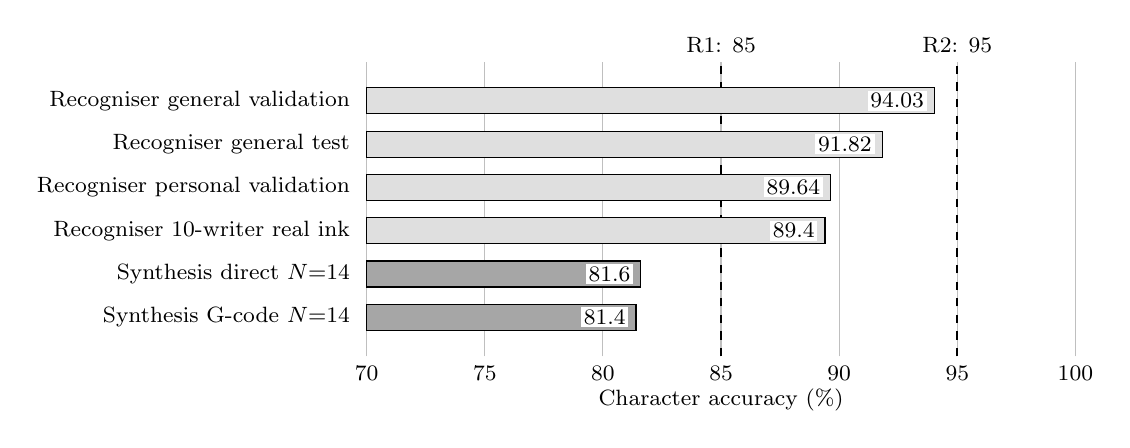
\begin{tikzpicture}[x=0.3cm,y=0.55cm]
\foreach \v in {70,75,80,85,90,95,100}{
  \draw[gray!50] ({\v-70},-0.4) -- ({\v-70},6.4);
  \node[font=\footnotesize,below] at ({\v-70},-0.4) {\v};
}
\node[font=\footnotesize] at (15,-1.4) {Character accuracy (\%)};
\draw[thick,dashed] (15,-0.4) -- (15,6.4);
\draw[thick,dashed] (25,-0.4) -- (25,6.4);
\node[font=\footnotesize,above] at (15,6.4) {R1: 85};
\node[font=\footnotesize,above] at (25,6.4) {R2: 95};
\foreach \lab/\val/\circ [count=\i from 0] in {Recogniser general validation/94.03/0,Recogniser general test/91.82/0,Recogniser personal validation/89.64/0,Recogniser 10-writer real ink/89.4/0,Synthesis direct $N{=}14$/81.6/1,Synthesis G-code $N{=}14$/81.4/1}{
  \pgfmathsetmacro{\yy}{5.5-\i}
  \ifnum\circ=1 \fill[gray!70] (0,{\yy-0.3}) rectangle ({\val-70},{\yy+0.3});
  \else \fill[gray!25] (0,{\yy-0.3}) rectangle ({\val-70},{\yy+0.3}); \fi
  \draw (0,{\yy-0.3}) rectangle ({\val-70},{\yy+0.3});
  \node[font=\footnotesize,anchor=east] at (-0.3,\yy) {\lab};
  \node[font=\footnotesize,anchor=east,fill=white,inner sep=1pt] at ({\val-70-0.3},\yy) {\val};
}
\end{tikzpicture}
\caption{Established character accuracies against the targets of R1 and R2. Light bars: recogniser on the general benchmark and on personal or real-ink data (optimistic splits). Dark bars: synthesised text read by the search judge (circular). The axis starts at 70\%.}
\label{fig:res-bars}
\end{figure}

        \QualificationSection{Observations}

            The circular figures for synthesised text (81.4\% to 81.6\% at $N=14$) lie below 85\%, whereas the server's stored figures (85.8\%, 84.1\%) and the scoped run (92.9\%) lie at or above it; these were obtained with different sentences, writers, tries and sample sizes.
            The genuine handwriting of the scoped run was read at 65.0\% and the synthesised text at 88.2\%.
            No independent evaluation, human panel or overlay distance exists.

        \QualificationSection{Statistical analysis}

            Intervals follow Equation~\ref{eq:res-wilson} and the bootstrap (over pages, writers and matched pairs); the pass criterion is a lower 95\% bound of at least 0.85 for $A_{\mathrm{c}}$ and $\rho$.
            \emph{Expected outcome.}
            Geometric features (slant, character width, ascender/descender ratio) are expected to correlate, because the synthesiser reuses the writer's own letter paths; stroke width and ink density are expected to deviate, because the plotter pen has one line width, so $\rho$ is reported with and without them.
            Overlay distances are expected to be dominated by spacing differences, so the AUC is expected to be clearly above 0.5 but well below 1.0; no numerical outcome is predicted.
            If the independent accuracy is below the circular figures, the quality setting and scoring weights must be re-tuned with an independent judge.

%%%%%%%%%%%%%%%%%%%%%%%%%%%%%%%%%%%%%%%%%%%%%%%%%%%%%%%%%%%%%%%%%%%%%%%%%%%%%%%%%

\medskip
    \QualificationTest{Classification of text and writer from real photographed pages (R2)}
\label{sec:res-qtp2}

        \QualificationSection{Objectives of the test or experiment}

            The test is to prove an overall accuracy of at least 95\% through the whole chain on pages never used for training, checkpoint selection or tuning.
            As the proposal does not define ``overall'', text accuracy $A_{\mathrm{c}}$ (Equation~\ref{eq:res-cacc}) and writer accuracy $A_{\mathrm{w}}$ (fraction of pages assigned to the correct writer) are reported separately and combined as
            \begin{equation}
            \label{eq:res-overall}
            A_{\mathrm{mean}}=\tfrac{1}{2}\left(A_{\mathrm{c}}+A_{\mathrm{w}}\right),\qquad A_{\mathrm{prod}}=A_{\mathrm{c}}\,A_{\mathrm{w}},
            \end{equation}
            where $A_{\mathrm{prod}}$ (both correct) is the criterion and $A_{\mathrm{mean}}$ the lenient reading.

        \QualificationSection{Equipment used}

            The capture rig, the ODROID N2+ with the final server and models, and a printed predefined paragraph; camera and lamp: \textbf{[TO BE COMPLETED BY STUDENT: camera model, resolution, mounting height, lamp type and photograph of the rig]}.

        \QualificationSection{Test setup and experimental parameters}

            The line-level validation split of the personal writers leaks: a random 15\% of lines per page was held out, so lines from the same sheet and session are in both sets (52 of 123 validation lines share pages with training), and the checkpoint was selected on them.
            The fix is new pages kept aside: at least 3 per personal writer, plus the held-out form page of each of the eight database writers, printed and photographed with the rig (about 14 pages, 350 lines).
            Seen lines are scored separately to quantify the leakage; references are double-entered transcripts.

        \QualificationSection{Steps followed in the test or experiment}

            Each frozen photograph is classified through the server without intervention; line text, per-line probabilities and the page-level mean probabilities are recorded, scored, summarised in a $10\times10$ confusion matrix, and the predefined paragraph is then classified live.

        \QualificationSection{Results or measurements}

            Table~\ref{tab:res-r2} lists the established figures, which come from splits that favour the system.

\begin{table}[h]
\centering
\fontsize{10}{12}\selectfont
\begin{tabularx}{\linewidth}{|>{\raggedright\arraybackslash}p{4.3cm}|>{\raggedright\arraybackslash}X|}
\hline
\textbf{Measure} & \textbf{Established figure and caveat, or status} \\
\hline
Recogniser, general benchmark & Validation 94.03\%, test 91.82\% character accuracy (reproduced exactly during analysis); word error rate 21.1\% / 26.7\%. Only the test figure is untouched by checkpoint selection. \\
\hline
Recogniser, personal validation lines & 89.64\%; 15\% of lines per page, optimistic. \\
\hline
Recogniser, 10-writer real ink & 89.4\%; not a clean unseen-writer test. \\
\hline
Writer classifier (ink), real validation pages & 100\%; line-level split inside pages, best checkpoint reported, no separate test set. \\
\hline
Shape classifier, real ink & 96.7\% (119 of 123 lines); the ink classifier reaches about 20\% on synthesised output. \\
\hline
Live check, one personal photograph & Correct writer at 98.6\% confidence, 28 lines detected, accurate transcription (single page, not a statistic). \\
\hline
Held-out pages ($A_{\mathrm{c}}$, $A_{\mathrm{w}}$, $A_{\mathrm{mean}}$, $A_{\mathrm{prod}}$, confusion matrix), paragraph demonstration & \nym{} \\
\hline
\end{tabularx}
\caption{Results for qualification test 2 (design-stage figures, not re-run for this report).}
\label{tab:res-r2}
\end{table}

        \QualificationSection{Observations}

            The recogniser reached 91.82\% (test) and 94.03\% (validation), 3.2 and 1.0 points below 95\%, and 89.64\% on personal lines.
            The word error rates (21.1\%, 26.7\%) are far higher than the character error rates (5.97\% to 8.18\%).
            The shape classifier made four errors on 123 lines.
            No overall accuracy on held-out photographed pages has been measured.

        \QualificationSection{Statistical analysis}

            With 14 pages, a perfect $A_{\mathrm{w}}$ has a Wilson lower bound of only about 78\%, and about 73 error-free pages would be needed for a bound of 95\%; the roughly 350 lines (lower bound about 98.9\% when error-free) are therefore reported as the more powerful but correlated statistic.
            \emph{Expected outcome.}
            Text accuracy on unseen personal handwriting is expected to be below the general-benchmark figure, because only 13 personal pages were available for fitting, so 95\% is not expected for text.
            If $A_{\mathrm{w}}$ is near 100\%, $A_{\mathrm{mean}}$ can exceed 95\% while $A_{\mathrm{prod}}$ does not.
            The writer accuracy on new pages is expected to fall below 100\%, since the ink classifier is sensitive to pen, paper and illumination.

%%%%%%%%%%%%%%%%%%%%%%%%%%%%%%%%%%%%%%%%%%%%%%%%%%%%%%%%%%%%%%%%%%%%%%%%%%%%%%%%%

\medskip
    \QualificationTest{Reproduction time per character (R3)}
\label{sec:res-qtp3}

        \QualificationSection{Objectives of the test or experiment}

            The test is to prove that a sentence of $x$ characters is reproduced within $4x$ seconds,
            \begin{equation}
            \label{eq:res-r3}
            t_{\mathrm{char}}=\frac{T_{\mathrm{syn}}+T_{\mathrm{write}}}{x}\le 4\ \mathrm{s},
            \end{equation}
            where $T_{\mathrm{syn}}$ is the synthesis time, $T_{\mathrm{write}}$ the time from first to last motion and $x$ the number of characters.
            As the proposal does not say whether synthesis counts, both variants are reported; calibration is a one-off step and is reported separately.

        \QualificationSection{Equipment used}

            The ODROID N2+ with the server, the assembled gantry, a stopwatch and logged time stamps at the start and end of synthesis and motion.

        \QualificationSection{Test setup and experimental parameters}

            Tries $N\in\{1,3,6,14,30\}$, sentences of 10, 20, 40 and 80 characters, 5 repetitions (100 syntheses); writing time for the 20 jobs at $N=14$.
            Only figures measured on the ODROID N2+ itself count; laptop figures are indicative.

        \QualificationSection{Steps followed in the test or experiment}

            After one calibration, each job is synthesised, sent and timed by log and stopwatch, $t_{\mathrm{char}}$ is computed from Equation~\ref{eq:res-r3}, and any stall is kept as a failed run.

        \QualificationSection{Results or measurements}

            Table~\ref{tab:res-r3} lists the established figures (laptop and generator model, not valid for the ODROID N2+).

\begin{table}[h]
\centering
\fontsize{10}{12}\selectfont
\begin{tabularx}{\linewidth}{|>{\raggedright\arraybackslash}p{4.5cm}|>{\raggedright\arraybackslash}X|}
\hline
\textbf{Measure} & \textbf{Established figure and caveat, or status} \\
\hline
Best-of-$N$ synthesis, 38 characters, server, loaded laptop & About 105~s (2.8~s per character); text read-back 97.4\%; $N$ not recorded. \\
\hline
Synthesis with 3 tries, laptop & About 5 to 7~s (sentence length not recorded). \\
\hline
Writing time, generator model (11-character word) & 2.4 to 2.8~s per character, about 34\% of it pen dwell; model values only. \\
\hline
Synthesis and writing time on the ODROID N2+; $t_{\mathrm{char}}$ against $N$ and $x$ & \nym{} \\
\hline
\end{tabularx}
\caption{Results for qualification test 3 (laptop and model figures only).}
\label{tab:res-r3}
\end{table}

        \QualificationSection{Observations}

            The laptop synthesis was below 4~s per character, and the 3-try synthesis took far less time (sentence lengths not recorded as equal).
            The model writing time added to the laptop synthesis time exceeds 4~s per character.
            The driver runs pen-up moves at the pen-down feed (single modal feed register), so the real writing time differs from the model.

        \QualificationSection{Statistical analysis}

            Mean, standard deviation and maximum of $t_{\mathrm{char}}$ over 5 repetitions are given per cell and the requirement is tested on the maximum; $T_{\mathrm{syn}}=a+bNx$ is fitted by regression.
            \emph{Expected outcome.}
            Each try renders and scores a candidate, so $T_{\mathrm{syn}}$ should grow linearly with $N$, and the ARM processor is expected to be slower than the laptop by an unmeasured factor.
            R3 is therefore expected to be met at few tries or for writing time alone, and not at $N=14$ if both are added, unless pen dwell, pen-up feed and search cost are reduced (Section~\ref{sec:discussion}).

%%%%%%%%%%%%%%%%%%%%%%%%%%%%%%%%%%%%%%%%%%%%%%%%%%%%%%%%%%%%%%%%%%%%%%%%%%%%%%%%%

\medskip
    \QualificationTest{Classification time (R4)}
\label{sec:res-qtp4}

        \QualificationSection{Objectives of the test or experiment}

            The test is to prove that the time from instruction to displayed text and writer satisfies
            \begin{equation}
            \label{eq:res-r4}
            T_{\mathrm{cls}}\le 2+0.025\,x\ \text{seconds},
            \end{equation}
            where $x$ is the number of handwritten characters; the stage times identify any shortfall.

        \QualificationSection{Equipment used}

            The rig, the ODROID N2+ with the final server, a logging wrapper (monotonic clock) around each stage and a stopwatch; the interface does not display classification time.

        \QualificationSection{Test setup and experimental parameters}

            Pages with $x=40$, about 200 and about 1000, each run 10 times; the budgets are 3.0, 7.0 and 27.0~s.
            Stages: capture, conditioning and segmentation, recognition per line, writer classification, display; the segmentation profile is repeated on the ODROID N2+.

        \QualificationSection{Steps followed in the test or experiment}

            The clocks start at the instruction, stage times and the total are logged, $x$ is counted from the transcript and Equation~\ref{eq:res-r4} is evaluated.

        \QualificationSection{Results or measurements}

            Table~\ref{tab:res-r4} lists the established figures (development laptop, not the ODROID N2+).

\begin{table}[h]
\centering
\fontsize{10}{12}\selectfont
\begin{tabularx}{\linewidth}{|>{\raggedright\arraybackslash}p{4.5cm}|>{\raggedright\arraybackslash}X|}
\hline
\textbf{Measure} & \textbf{Established figure and caveat, or status} \\
\hline
Segmentation of one $2400\times1800$ photograph, pure Python, laptop & 35 to 57~s (loaded at times); line grouping and chain search dominated (about 70\% in the cleanest run), then labelling and box-filter blurs. \\
\hline
Same with two routines in C99 & About 25\% to 32\% faster end to end; the C routines are 84\% to 88\% faster than their Python versions; optional, not deployed. \\
\hline
Recogniser on a PC & 2.6 to 3.1~s per line, about 65 to 75~ms per character. \\
\hline
Capture, classification and total on the ODROID N2+; $T_{\mathrm{cls}}$ for $x=40$, 200, 1000 & \nym{} \\
\hline
\end{tabularx}
\caption{Results for qualification test 4 (laptop figures only).}
\label{tab:res-r4}
\end{table}

        \QualificationSection{Observations}

            Segmentation took 17 to 28 times the 2~s budget in pure Python (12 to 21 times with the C routines).
            For a 40-character line the allowance is 3.0~s, whereas segmentation alone took at least 35~s and recognition about 2.6 to 3.0~s.
            The recogniser time per character is 2.6 to 3.0 times the specified 25~ms.

        \QualificationSection{Statistical analysis}

            Mean, standard deviation, maximum and stage shares over 10 repetitions are reported; the requirement is tested on the maximum.
            \emph{Expected outcome.}
            The ARM processor is expected to be slower than the laptop, so the shortfall on the target is expected to be at least as large, dominated by segmentation; the budget cannot be met without the redesign of Section~\ref{sec:discussion}.
            Recognition alone ($1000\times0.065=65$~s) is expected to miss the full-page budget of 27~s.

%%%%%%%%%%%%%%%%%%%%%%%%%%%%%%%%%%%%%%%%%%%%%%%%%%%%%%%%%%%%%%%%%%%%%%%%%%%%%%%%%

\medskip
    \QualificationTest{Absolute positional accuracy of the gantry (R5)}
\label{sec:res-qtp5}

        \QualificationSection{Objectives of the test or experiment}

            The test is to prove that the absolute positional error of drawn marks is at most 0.5~mm and that a word written twice coincides within that tolerance.
            Software contributions (quantisation, calibration) and hardware contributions (mechanics, homing repeatability, pen compliance) are separated.

        \QualificationSection{Equipment used}

            The gantry with pen and paper, a flat-bed scanner (600 dots per inch, 0.042~mm per pixel), a steel ruler or vernier calipers (0.02~mm) and a printed calibration sheet with a 10~mm grid of crosses.

        \QualificationSection{Test setup and experimental parameters}

            Software part (offline): the step is $1/80=12.5~\mu$m, the quantisation error per axis at most $6.25~\mu$m and the combined worst case $8.8~\mu$m (derived).
            Hardware part: at least 40 crosses drawn 5 times after fresh calibrations, the paper fixed against registration stops, and the same word written twice.
            The error of a cross is $e_i=\lVert\mathbf{p}_i-\mathbf{p}_i^{\mathrm{cmd}}\rVert$ (measured against commanded position referenced to the machine origin); mean, maximum and 95th percentile are reported with the measurement uncertainty (Equations~\ref{eq:res-r5} and~\ref{eq:res-unc} in the Appendix).

        \QualificationSection{Steps followed in the test or experiment}

            After calibration (the direction pin must be seen to change level on reversal) the grid is drawn, scanned with the ruler, evaluated by image analysis, repeated 5 times, and the overlay of the word written twice is produced (Appendix).

        \QualificationSection{Results or measurements}

            Resolution and quantisation values are derived, not measured; all physical measurements are \nym{}.
            During bring-up the X-axis calibration reached the first end-stop, but the direction pin (physical pin 7) was not observed to change level on reversal; this fault was unresolved and is under investigation.

        \QualificationSection{Observations}

            No positional measurement exists.
            The only hardware observation is the direction-pin fault.
            The digital resolution is 40 times finer than the 0.5~mm tolerance.

        \QualificationSection{Statistical analysis}

            The maximum, mean and 95th percentile of $e_i$ over at least 200 points are given with a bootstrap interval; a pass requires the maximum to be at most 0.5~mm, and a result within twice the expanded uncertainty of the limit is inconclusive.
            \emph{Expected outcome.}
            The software contribution is negligible; the error is expected to be dominated by open-loop effects (lost steps, belt stretch, backlash, switch repeatability, pen compliance), none of which has been measured.
            The literature value of 0.3~mm \cite{huang2024} leaves a 0.2~mm margin.
            The test grid must lie within the common work area, since the generator area (200~mm) exceeds the driver's travel (194~mm in X).

%%%%%%%%%%%%%%%%%%%%%%%%%%%%%%%%%%%%%%%%%%%%%%%%%%%%%%%%%%%%%%%%%%%%%%%%%%%%%%%%%

\medskip
    \QualificationTest{Multi-writer storage (R6)}
\label{sec:res-qtp6}

        \QualificationSection{Objectives of the test or experiment}

            The test is to prove that at least 10 writing styles are stored permanently and that any can be selected at random for reproduction.

        \QualificationSection{Equipment used}

            The ODROID N2+ with the server, a laptop browser and the gantry.

        \QualificationSection{Test setup and experimental parameters}

            The eight database and two personal writers; file counts and sizes; persistence by restarting the server and power-cycling the board; 3 writers drawn with a fixed seed.

        \QualificationSection{Steps followed in the test or experiment}

            The listed writers are compared with the stored files, the list is re-read after restart and power cycle, and a short sentence is written in each of the 3 drawn styles.

        \QualificationSection{Results or measurements}

            The server listed 10 writers in a live check; each is stored as a JSON profile with trained weights; sizes: \textbf{[TO BE COMPLETED BY STUDENT: size of each profile and of the weight files]}.
            Persistence and the gantry demonstration are \nym{}.

        \QualificationSection{Observations}

            The list contained 10 entries, equal to the minimum.

        \QualificationSection{Statistical analysis}

            This is a count and pass/fail test; no statistical analysis is appropriate.
            \emph{Expected outcome.}
            Persistence is expected because the profiles are files; the gantry demonstration depends on the fault of qualification test 5.

%%%%%%%%%%%%%%%%%%%%%%%%%%%%%%%%%%%%%%%%%%%%%%%%%%%%%%%%%%%%%%%%%%%%%%%%%%%%%%%%%

\subsubsection*{Field condition checks (FC1 and FC2)}
\label{sec:res-fc}

Neither field condition was measured.
\textbf{FC1:} a lux meter at the page plane records five points (centre and corners of an A4 page); the condition is met if all lie between 400 and 1000~lux, and qualification test 2 is repeated on the same pages at about 200, 700 and 1200~lux.
Illuminance: \nym{}; the flat-field correction and local thresholding should limit degradation within the range, with larger degradation below 400~lux.
\textbf{FC2:} a spirit level or inclinometer on both axes (tilt below $0.5^\circ$) and a logging accelerometer on the frame during a standard job, with the repeat error of qualification test 5 at rest and with a lightly tapped bench.
Tilt and vibration: \nym{}.

